\scanpage{33}
\margin{32}

La subdivision barycentrique de $C$, qui est aussi celle de $C^*$, est apparente sur la description donnée, ses faces sont les drapeaux qui ont servi de composants pour la construction des $\operatorname{Dis}_s=|\vec A_s|$. (Cf traits \figure{\begin{tikzpicture}[baseline=-.5ex]\draw[green!40!black,thick](0,0)--(.6,0);\draw[yellow!65!green,thick](.8,0)--(1.4,0);\draw[dashed](1.6,0)--(2.2,0);\end{tikzpicture}})

On va donner une autre construction, de la surface $\mathcal X$ sous-jacente à $C$, qui s'obtient intuitivement en \unsure{traçant|tirant} des petits disques \deleted{\unsure{les}} autour des sommets de la \deleted{face} \inserted{carte} duale, \inserted{(centres des faces de $C$)} et \unsure{enlevant|incluant} les portions d'arêtes de $C^*$ (bleues) qui se trouvent à l'intérieur. La \uline{surface à bord} déduite de $\unsure{C^a|C^*}$ en enlevant les disques, avec la décomposition cellulaire définie par la construction précédente (dont les faces de $\unsure{C'}$ étant \unsure{réalisées|représentées} par les $\operatorname{Dis}_s$ ($s\in S$)), s'obtient en remplaçant les $\operatorname{Dis}_s$ par les $\operatorname{Dis}'_s$, obtenus en ``enlevant les coins'' de ces plaques polygonales. Chaque $\vec A_s$ est remplacé par le polygone combinatoire ``doublé'' $\unsure{\vec A'_s}$ (\deleted{\unsure{l'ens des sommets}} \inserted{dont les \deleted{sommets} arêtes sont les} repères de $\vec A_s$), \deleted{dont le} d'ordre $\unsure{2\nu}$, et en prenant le polygone dual, dont les ``arêtes'' \inserted{\unsure{d'inertie}} sont en corr. biunivoque avec les \deleted{repères} \inserted{arêtes de $\vec A_s$} \deleted{de $\vec A_s$}, et les ``arêtes de recollement'' avec les \deleted{\unsure{qui sont les repères, c'est les sommets}} \inserted{sommets de $\vec A_s$} \deleted{\unsure{qui sont}}. Ceci dit, en recollant les $\operatorname{Dis}_s$ ($s\in S$) suivant les arêtes de recollement seulement, on trouve une carte à bord dont les faces sont les $\operatorname{Dis}'_s$, et les comp. connexes du bord sont en corr. $1-1$ avec l'ens des faces de $C$ i.e. les sommets de $C^*$ --- donc ce sont les orbites sous le groupe diédral $\langle\sigma_1,\sigma_0\rangle$ contenant $\langle\rho_f\rangle$ comme un sous-groupe d'indice (1 ou) 2. Notons que dans le procédé de recollement précédent, chaque composante connexe \deleted{\unsure{d'inertie|d'intérieur}} du bord apparaît comme un polygone topologique, \unsure{d'indice égal à l'ordre|l'indice égale l'ordre}

\figure{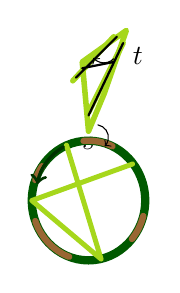
\begin{tikzpicture}[x=.8cm,y=.8cm,line cap=round,line join=round]
\draw[yellow!65!green,line width=2pt] (0,1.1)--(-.1,2.2)--(.6,2.7)--(.25,1.7)--cycle;
\draw[yellow!65!green,line width=2pt] (-.25,1.9)--(.4,2.6) (0,1.4)--(.55,2.5);
\draw[black,thick] (-.2,1.95)--(.45,2.6) (0,1.35)--(.55,2.5) (-.1,2.1)--(.4,2.2);
\draw[black,->] (.4,2.25)arc(-45:-140:.22);\node[right]at(.55,2.3){$t$};\node[below]at(0,1.15){$s$};
\draw[green!35!black,line width=3pt] (0,0) ellipse(.9 and .95);
\draw[yellow!65!green,line width=1.8pt] (-.35,.88)--(.2,-.93) (-.9,0)--(.7,.58) (-.9,0)--(.2,-.93);
\draw[brown!80!black,line width=2.3pt] (65:.9 and .95)arc(65:95:.9 and .95) (145:.9 and .95)arc(145:160:.9 and .95) (200:.9 and .95)arc(200:250:.9 and .95) (-15:.9 and .95)arc(-15:-40:.9 and .95);
\draw[green!20!black,very thick,->] (-.4,.85)arc(120:170:.85);\draw[black,->] (.15,1.2)arc(80:-45:.2);
\end{tikzpicture}}

\diagram{\begin{array}{lllll}
\texttt{PAGE 1}&\texttt{ON=CELMPQRSTV}&\texttt{08/19/82-15:06:51}&\texttt{CFT 1.09(06/28/82)}&\texttt{PAGE 1}
\end{array}}
\diagram{\begin{array}{rrl}
\texttt{1}&\texttt{1.}&\texttt{PROGRAM CRAY7}\\
\texttt{2}&\texttt{2.}&\texttt{WRITE(6,1)}\\
\texttt{3}&\texttt{3.}&\texttt{1 FORMAT(' BONJOUR')}\\
\texttt{4}&\texttt{4.}&\texttt{STOP}\\
\texttt{5}&\texttt{5.}&\texttt{END}
\end{array}}
